% =============================================================================
% 5 Modellbildung und Plausibilisierung des thermischen Drifts
% =============================================================================
\section{Modellbildung und Plausibilisierung des thermischen Drifts}
\label{chap:modellbildung}

In Kapitel~\ref{chap:analyse_pruefstand} wurde die Erwärmung der
V2A-Lastwiderstände als wesentliche Ursache für die zeitliche Abnahme der
Modulströme identifiziert. Mit zunehmender Temperatur steigt der elektrische
Widerstand der V2A-Schienen. Bei näherungsweise konstanter Klemmenspannung
sinkt dadurch der Strom des betreffenden Lastzweigs. Ziel dieses Kapitels ist
es, diese elektrothermische Wirkung in einem nachvollziehbaren Simulationsmodell
abzubilden und die Größenordnung des zu erwartenden Stromdrifts zu bestimmen.

Das Modell wird schrittweise aufgebaut. Ausgehend von einem thermischen
System erster Ordnung werden zunächst die physikalischen Modellparameter
eingeführt und anschließend die elektrische und thermische Domäne gekoppelt.
Die mathematische Herleitung, die Umsetzung in MATLAB/Simulink und die
Plausibilisierung anhand analytisch bestimmbarer Grenzfälle werden gemeinsam
dargestellt. Gegenstand ist ausschließlich der Drift eines einzelnen
V2A-Lastzweigs. Die in Kapitel~\ref{chap:konzeptentwicklung} entwickelte
Nachregelung mit Trafo~2 und Stellwiderstand wird an dieser Stelle noch nicht
modelliert.


% -----------------------------------------------------------------------------
% 5.1 Zielsetzung, Systemgrenze und Modellannahmen
% -----------------------------------------------------------------------------
\subsection{Zielsetzung, Systemgrenze und Modellannahmen}
\label{sec:zielsetzung_systemgrenze_modellannahmen}

Die Systemgrenze umfasst die Klemmenspannung eines MCC-Abgangs, den daran
angeschlossenen V2A-Lastwiderstand und dessen Wärmeabgabe an die Umgebung. Als
Ausgangsgrößen werden die Temperatur des Widerstands, sein elektrischer
Widerstand, der Laststrom und die umgesetzte elektrische Leistung betrachtet.
Die vorgelagerte Einspeisung, die übrigen elf MCC-Abgänge, das
Leistungsschalterfeld und die Kurzschlussbrücke liegen außerhalb der
Systemgrenze. Damit wird nicht der vollständige Prüfstand, sondern gezielt der
für den thermischen Stromdrift maßgebende Wirkzusammenhang untersucht.

Für die Modellbildung werden folgende Annahmen getroffen:

\begin{itemize}
    \item Der V2A-Widerstand wird als konzentrierter thermischer Körper mit
          räumlich homogener Temperatur beschrieben.
    \item Die Materialkennwerte, die wirksame Oberfläche und der
          Wärmeübergangskoeffizient werden innerhalb eines Simulationsfalls als
          konstant angenommen.
    \item Die Wärmeabgabe wird durch einen zusammengefassten thermischen
          Widerstand gegenüber einer konstanten Umgebungstemperatur erfasst.
    \item Die Spannung am Lastzweig wird nach dem Einschaltzeitpunkt als
          idealer Spannungssprung vorgegeben.
    \item Leitungs-, Kontakt- und Modulwiderstände werden gegenüber dem
          einstellbaren V2A-Widerstand vernachlässigt. Diese Widerstände werden
          somit nicht als physikalisch null bewertet, sondern im Sinne einer
          gezielten Modellreduktion außerhalb der Systemgrenze belassen.
    \item Magnetische, dreiphasige und gegenseitige thermische Kopplungen
          zwischen den Abgängen werden nicht abgebildet.
\end{itemize}

Die Beschreibung eines Bauteils durch eine einzige Körpertemperatur ist nur
dann zulässig, wenn die innere Temperaturverteilung für die betrachtete
Fragestellung von untergeordneter Bedeutung ist. Für kleine beziehungsweise
thermisch gut leitende Körper wird dieses Vorgehen als konzentriertes
thermisches Modell verwendet \parencite[S.~30--33]{Griesinger_Waermemanagement}.
Bei den räumlich ausgedehnten V2A-Schienen ist diese Voraussetzung nicht über
den gesamten Körper streng erfüllt. Die Annahme dient hier daher der
Beschreibung des mittleren dynamischen Verhaltens und nicht der Ermittlung
lokaler Maximaltemperaturen.


% -----------------------------------------------------------------------------
% 5.2 Schrittweise Modellentwicklung und Modellreduktion
% -----------------------------------------------------------------------------
\subsection{Schrittweise Modellentwicklung und Modellreduktion}
\label{sec:modellentwicklung_modellreduktion}

Die Modellbildung erfolgte in drei aufeinander aufbauenden Stufen. In der
ersten Stufe wurde das thermische Grundverhalten normiert als PT1-System
umgesetzt. Abbildung~\ref{fig:modellstufe_1} zeigt die zugehörige Struktur. Die
zugeführte Wärmeleistung wird mit der abgeführten Wärmeleistung bilanziert; ein
Integrator bildet aus der verbleibenden Leistung die Temperaturänderung. Diese
Stufe dient vor allem der Kontrolle von Vorzeichen, Rückführung und
Einschwingverhalten.

\begin{figure}[H]
    \centering
    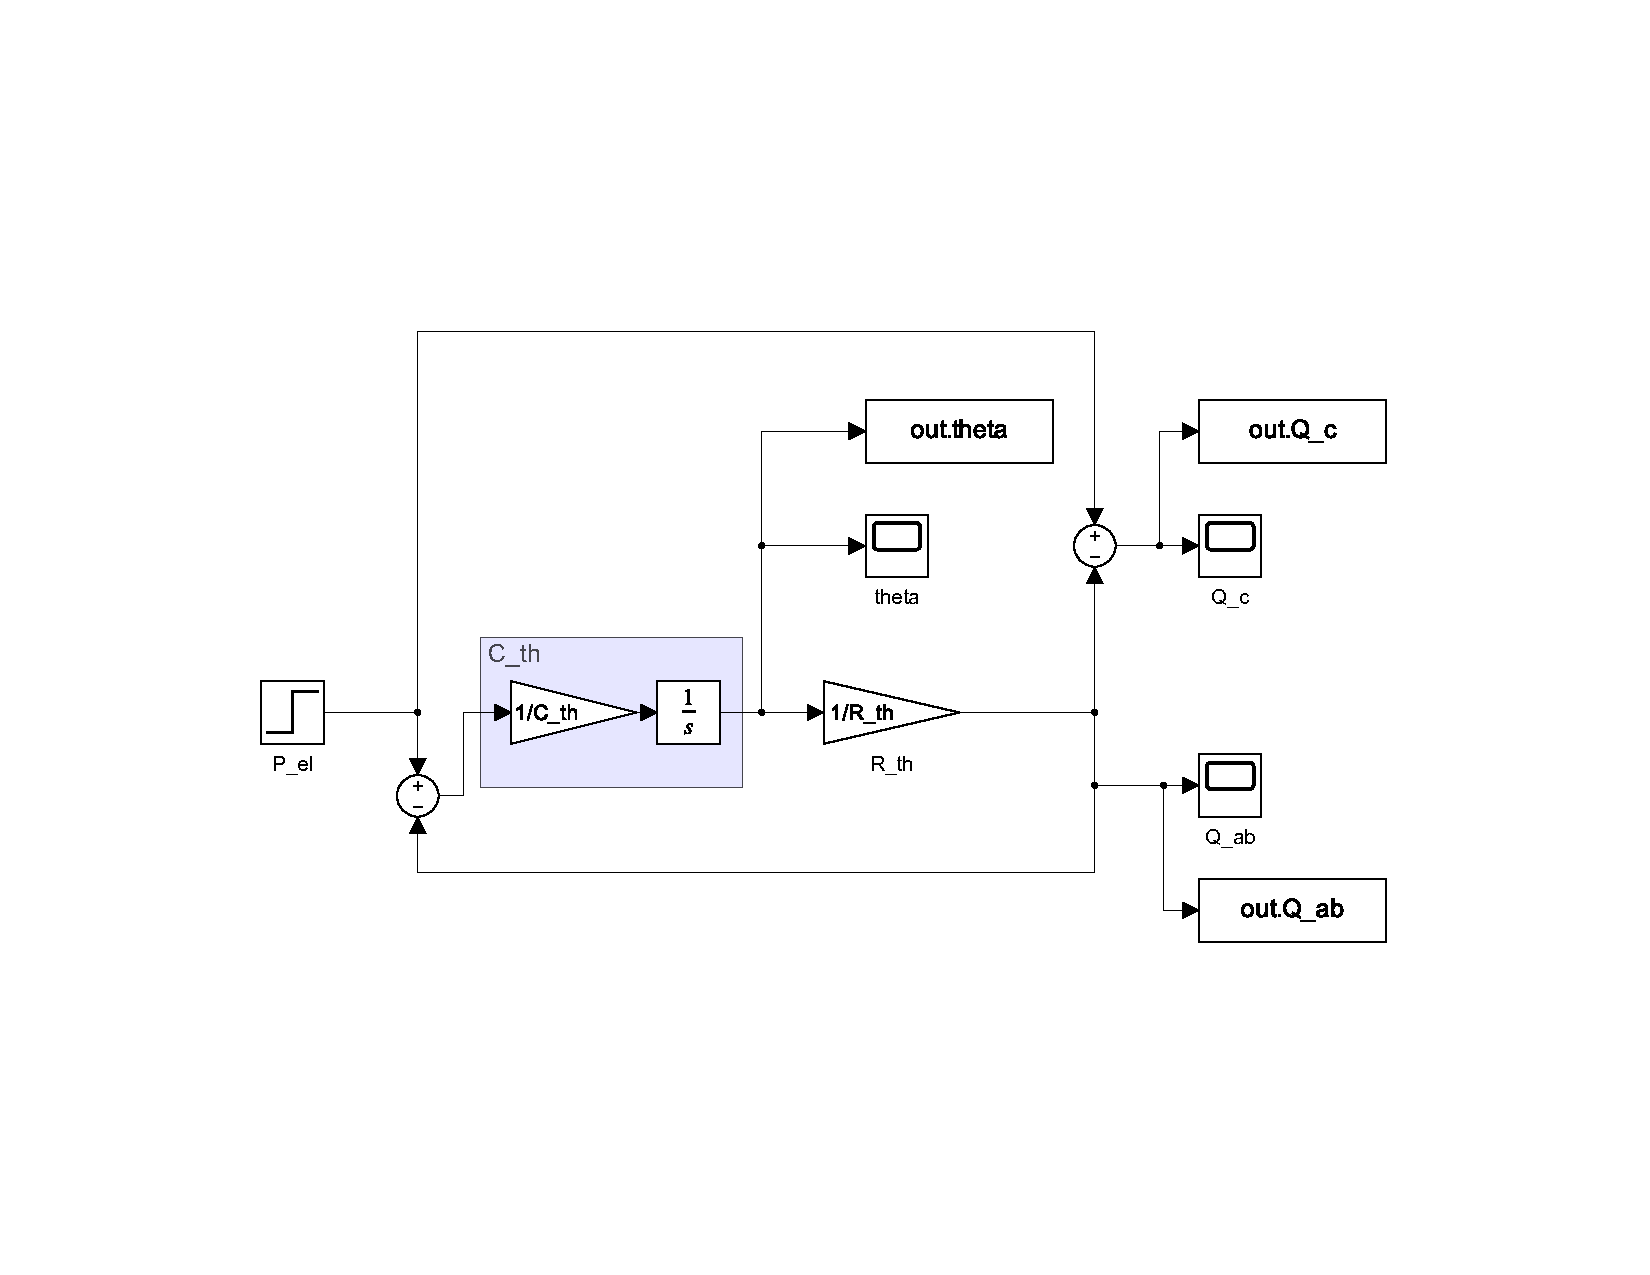
\includegraphics[width=0.95\textwidth,
        trim={3.2cm 4.0cm 3.2cm 4.0cm},clip]
    {03_Ressourcen/pic/RC_Modell_1.pdf}
    \caption{Erste Modellstufe: normiertes thermisches System erster Ordnung
    (eigene Darstellung in MATLAB/Simulink)}
    \label{fig:modellstufe_1}
\end{figure}

In der zweiten Stufe wurden die normierten Größen durch die physikalischen
Parameter Wärmekapazität, thermischer Widerstand und Umgebungstemperatur
ersetzt. Die elektrische Verlustleistung ist in dieser Stufe noch eine
unabhängig vorgegebene Eingangsgröße. Dadurch kann das thermische Teilmodell
isoliert geprüft werden, ohne dass eine fehlerhafte elektrische Rückkopplung
das Ergebnis beeinflusst.

\begin{figure}[H]
    \centering
    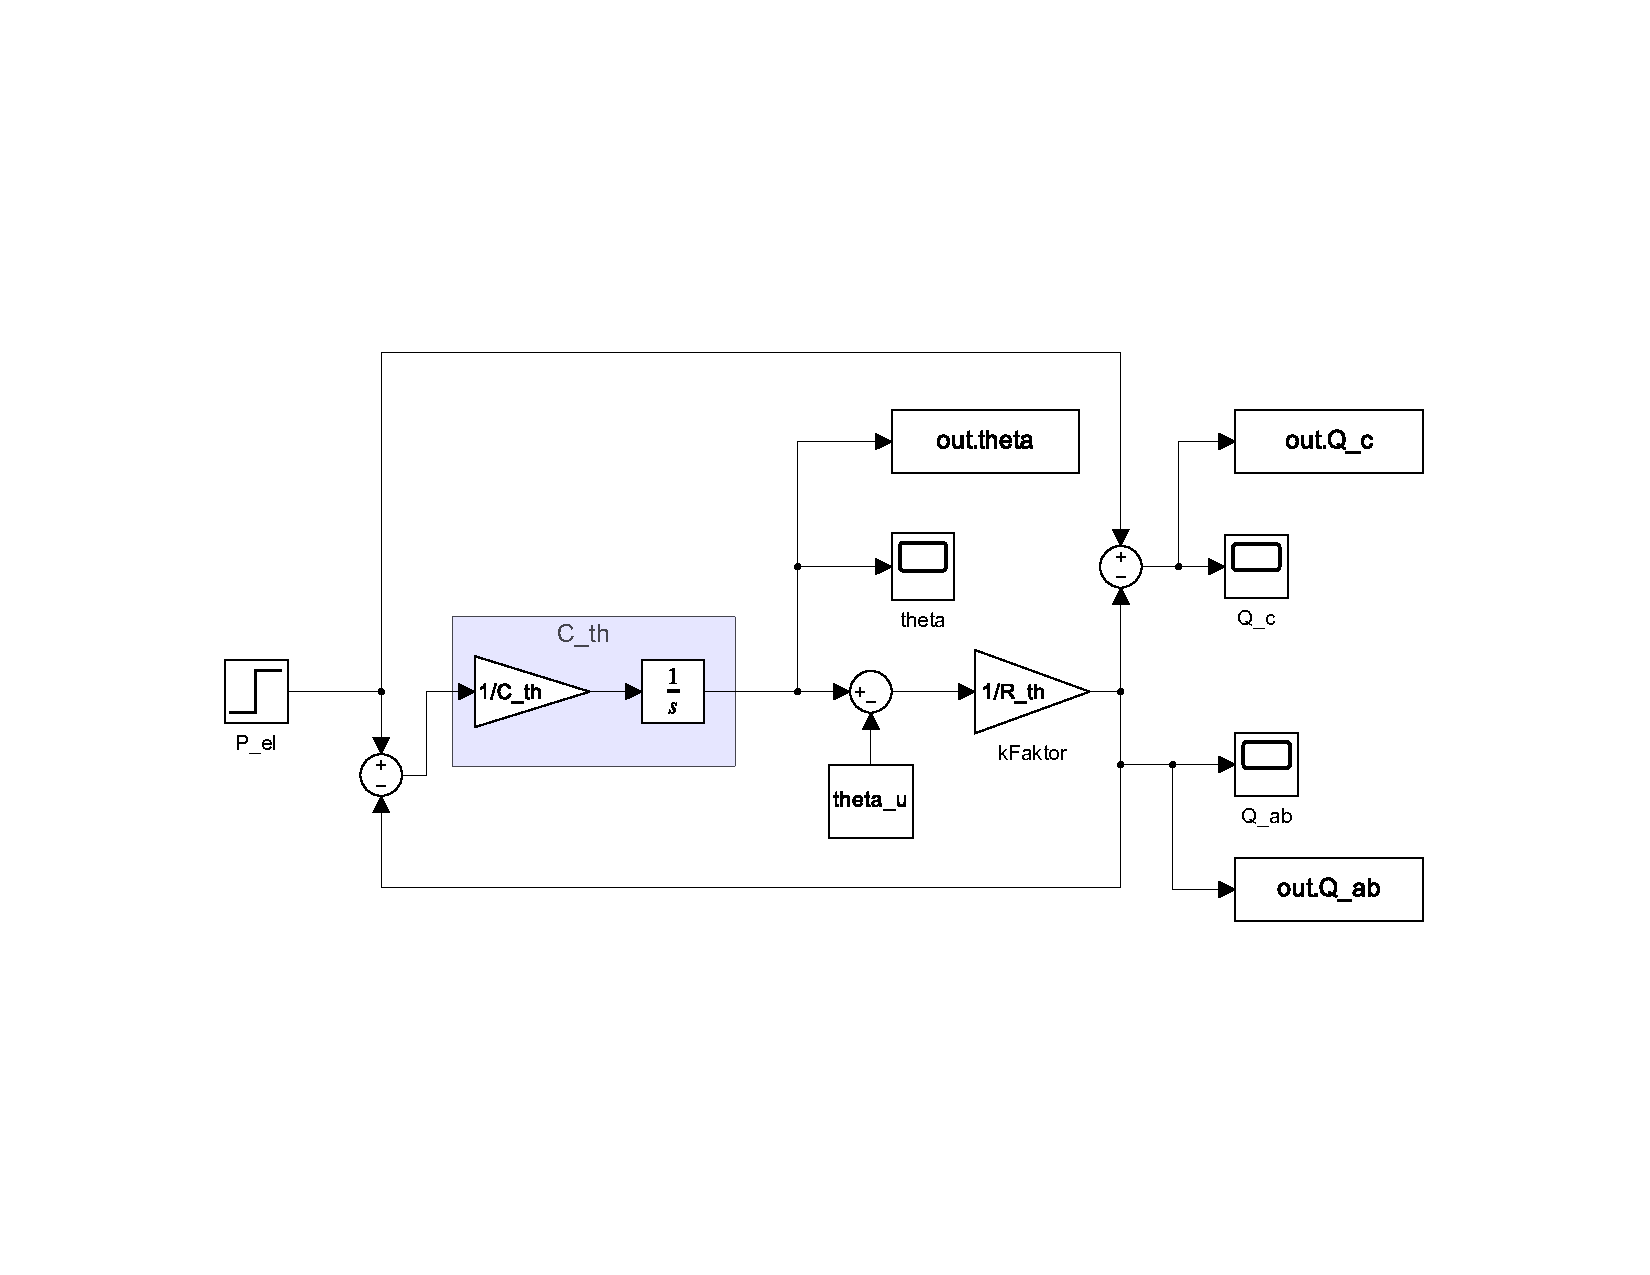
\includegraphics[width=0.95\textwidth,
        trim={3.2cm 4.0cm 3.2cm 4.0cm},clip]
    {03_Ressourcen/pic/RC_Modell_2.pdf}
    \caption{Zweite Modellstufe: thermisches Teilmodell mit physikalischen
    Parametern und vorgegebener Verlustleistung
    (eigene Darstellung in MATLAB/Simulink)}
    \label{fig:modellstufe_2}
\end{figure}

Die dritte Stufe schließt den elektrothermischen Wirkungskreis. Aus der
vorgegebenen Spannung und dem temperaturabhängigen Widerstand werden Strom und
Verlustleistung berechnet. Die Verlustleistung erwärmt den Widerstand, dessen
Temperatur wiederum auf den elektrischen Widerstand zurückwirkt. Diese
schrittweise Entwicklung ermöglicht es, Fehler zunächst einer Domäne
zuzuordnen und die Teilmodelle vor ihrer Kopplung getrennt zu plausibilisieren.


% -----------------------------------------------------------------------------
% 5.3 Modellierung der Spannungsquelle
% -----------------------------------------------------------------------------
\subsection{Modellierung der Spannungsquelle}
\label{sec:spannungsquelle_messwertaufbereitung}

Im realen Prüfstand wird die Spannung des Hochstromtransformators durch den
motorisch verstellten Säulenstelltransformator verändert. Eine detaillierte
Abbildung dieses Stellvorgangs würde zusätzliche, für die Untersuchung des
thermischen Drifts nicht benötigte Zeitkonstanten und Regelparameter erfordern.
Für die Simulation wird die Einspeisung deshalb auf eine ideale
Spannungsquelle reduziert. Der zeitliche Verlauf lautet

\begin{equation}
    u_{\mathrm{V2A}}(t)
    =
    U_{\mathrm{V2A}}\,H\!\left(t-t_{\mathrm{s}}\right),
    \label{eq:modell_spannungssprung}
\end{equation}

wobei \(H(t)\) die Heaviside-Funktion und \(t_{\mathrm{s}}\) den
Einschaltzeitpunkt bezeichnet. In den Simulationen wird der Sprung bei
\(t_{\mathrm{s}}=\SI{300}{\second}\) aufgeschaltet. Die ersten fünf Minuten
stellen damit einen eindeutig auswertbaren Anfangszustand her.

Der Spannungssprung wurde einer linearen Spannungsrampe vorgezogen, weil seine
Sprungantwort unmittelbar mit der analytischen Lösung des thermischen
PT1-Grundmodells verglichen werden kann. Eine Rampe würde das thermische
Einschwingen mit dem Hochfahren der Quelle überlagern und die Zuordnung von
Abweichungen erschweren. Der Sprung ist somit eine gezielte Prüfanregung des
Modells und keine Behauptung über den realen Einschaltvorgang des Prüfstands.


% -----------------------------------------------------------------------------
% 5.4 Elektrisches Teilmodell
% -----------------------------------------------------------------------------
\subsection{Elektrisches Teilmodell des V2A-Lastzweigs}
\label{sec:elektrisches_teilmodell}

Der betrachtete V2A-Widerstand wird geometrisch durch die wirksame Länge \(L\),
die Breite \(b\) und die Dicke \(d\) beschrieben. Für den elektrischen
Querschnitt gilt

\begin{equation}
    A_{\mathrm{q}}=b\,d.
    \label{eq:modell_elektrischer_querschnitt}
\end{equation}

Aus dem spezifischen elektrischen Widerstand bei
\SI{20}{\degreeCelsius} folgt der Bezugswiderstand

\begin{equation}
    R_{\mathrm{V2A},20}
    =
    \rho_{\mathrm{el},20}\frac{L}{A_{\mathrm{q}}}.
    \label{eq:modell_widerstand_20}
\end{equation}

Im untersuchten Temperaturbereich wird die Temperaturabhängigkeit linear
angenähert:

\begin{equation}
    R_{\mathrm{V2A}}\!\left(\vartheta_{\mathrm{V2A}}\right)
    =
    R_{\mathrm{V2A},20}
    \left[
        1+\alpha_{\mathrm{el}}
        \left(\vartheta_{\mathrm{V2A}}-\SI{20}{\degreeCelsius}\right)
    \right].
    \label{eq:modell_widerstand_temperatur}
\end{equation}

Mit der vorgegebenen Klemmenspannung ergeben sich der Strom und die im
Widerstand umgesetzte elektrische Leistung zu

\begin{align}
    I_{\mathrm{V2A}}(t)
    &=
    \frac{u_{\mathrm{V2A}}(t)}
         {R_{\mathrm{V2A}}\!\left(\vartheta_{\mathrm{V2A}}(t)\right)},
    \label{eq:modell_strom}\\
    P_{\mathrm{el}}(t)
    &=
    u_{\mathrm{V2A}}(t)I_{\mathrm{V2A}}(t)
     =
    \frac{u_{\mathrm{V2A}}^{2}(t)}
         {R_{\mathrm{V2A}}\!\left(\vartheta_{\mathrm{V2A}}(t)\right)}.
    \label{eq:modell_verlustleistung}
\end{align}

Damit ist die elektrische Verlustleistung nicht konstant. Sie nimmt bei
konstanter Spannung mit steigendem Widerstand ab. Diese Rückwirkung wird erst
im vollständig gekoppelten Modell wirksam.


% -----------------------------------------------------------------------------
% 5.5 Thermisches Teilmodell
% -----------------------------------------------------------------------------
\subsection{Thermisches Teilmodell des V2A-Widerstands}
\label{sec:thermisches_teilmodell}

Das Volumen und die Masse der wirksamen Widerstandsschienen werden mit

\begin{align}
    V_{\mathrm{V2A}} &= Lbd,
    \label{eq:modell_volumen}\\
    m_{\mathrm{V2A}} &= \rho_{\mathrm{m}}V_{\mathrm{V2A}}
    \label{eq:modell_masse}
\end{align}

bestimmt. Daraus folgt die thermische Kapazität

\begin{equation}
    C_{\mathrm{th}}
    =m_{\mathrm{V2A}}c_{p}.
    \label{eq:modell_waermekapazitaet}
\end{equation}

Für die wirksame Oberfläche werden die beiden großen und die beiden schmalen
Längsseiten berücksichtigt. Die Stirnflächen werden aufgrund ihres geringen
Anteils vernachlässigt:

\begin{equation}
    A_{\mathrm{O}}
    =2L(b+d).
    \label{eq:modell_oberflaeche}
\end{equation}

Konvektion und weitere nicht getrennt parametrierte Wärmeübergänge werden in
einem effektiven Wärmeübergangskoeffizienten \(\alpha_{\mathrm{K}}\)
zusammengefasst. Der thermische Widerstand gegenüber der Umgebung lautet damit

\begin{equation}
    R_{\mathrm{th}}
    =\frac{1}{\alpha_{\mathrm{K}}A_{\mathrm{O}}}.
    \label{eq:modell_thermischer_widerstand}
\end{equation}

Der Wärmeübergangskoeffizient hängt in der Realität unter anderem von
Geometrie, Strömungszustand, Temperatur und Einbaulage ab. Seine Verwendung als
konstanter Kennwert stellt deshalb eine Modellvereinfachung dar
\parencite[S.~37--41]{Griesinger_Waermemanagement}. Für die vorliegende
Parameterstudie wird \(\alpha_{\mathrm{K}}\) als effektiver Mittelwert
angesetzt.

Die zugeführte elektrische Leistung teilt sich in den im Körper gespeicherten
Wärmestrom und den an die Umgebung abgeführten Wärmestrom auf:

\begin{equation}
    P_{\mathrm{el}}(t)
    =
    \dot Q_{\mathrm{C}}(t)
    +
    \dot Q_{\mathrm{ab}}(t).
    \label{eq:modell_waermebilanz}
\end{equation}

Mit

\begin{align}
    \dot Q_{\mathrm{C}}(t)
    &=C_{\mathrm{th}}
      \frac{\mathrm{d}\vartheta_{\mathrm{V2A}}(t)}{\mathrm{d}t},
    \label{eq:modell_waermestrom_speicher}\\
    \dot Q_{\mathrm{ab}}(t)
    &=\frac{
        \vartheta_{\mathrm{V2A}}(t)-\vartheta_{\mathrm{u}}
      }{R_{\mathrm{th}}}
    \label{eq:modell_waermestrom_abgabe}
\end{align}

ergibt sich die thermische Differentialgleichung

\begin{equation}
    C_{\mathrm{th}}
    \frac{\mathrm{d}\vartheta_{\mathrm{V2A}}(t)}{\mathrm{d}t}
    =
    P_{\mathrm{el}}(t)
    -
    \frac{
        \vartheta_{\mathrm{V2A}}(t)-\vartheta_{\mathrm{u}}
    }{R_{\mathrm{th}}}.
    \label{eq:modell_thermische_dgl}
\end{equation}

Die bis zum Zeitpunkt \(t\) gespeicherte und abgeführte Wärmeenergie kann
durch Integration der zugehörigen Wärmeströme bestimmt werden:

\begin{align}
    Q_{\mathrm{C}}(t)
    &=\int_{0}^{t}\dot Q_{\mathrm{C}}(\tau)\,\mathrm{d}\tau,
    \label{eq:modell_waermeenergie_speicher}\\
    Q_{\mathrm{ab}}(t)
    &=\int_{0}^{t}\dot Q_{\mathrm{ab}}(\tau)\,\mathrm{d}\tau.
    \label{eq:modell_waermeenergie_abgabe}
\end{align}

Für eine konstante, von der Temperatur unabhängige Verlustleistung ist
Gleichung~\eqref{eq:modell_thermische_dgl} linear. Mit der Übertemperatur

\begin{equation}
    \Delta\vartheta(t)
    =\vartheta_{\mathrm{V2A}}(t)-\vartheta_{\mathrm{u}}
    \label{eq:modell_uebertemperatur}
\end{equation}

und verschwindender Anfangsübertemperatur folgt nach der
Laplace-Transformation

\begin{equation}
    C_{\mathrm{th}}s\,\Delta\Theta(s)
    =
    P_{\mathrm{el}}(s)
    -\frac{\Delta\Theta(s)}{R_{\mathrm{th}}}.
    \label{eq:modell_laplace_waermebilanz}
\end{equation}

Die Übertragungsfunktion zwischen Verlustleistung und Übertemperatur lautet
damit

\begin{equation}
    G_{\mathrm{th}}(s)
    =
    \frac{\Delta\Theta(s)}{P_{\mathrm{el}}(s)}
    =
    \frac{R_{\mathrm{th}}}
         {1+sR_{\mathrm{th}}C_{\mathrm{th}}}.
    \label{eq:modell_uebertragungsfunktion_pt1}
\end{equation}

Die thermische Zeitkonstante beträgt

\begin{equation}
    \tau_{\mathrm{th}}
    =R_{\mathrm{th}}C_{\mathrm{th}}.
    \label{eq:modell_zeitkonstante}
\end{equation}

Für eine konstante Verlustleistung und eine beliebige Anfangstemperatur ergibt
sich die Zeitfunktion

\begin{equation}
    \vartheta_{\mathrm{V2A}}(t)
    =
    \vartheta_{\mathrm{u}}
    +P_{\mathrm{el}}R_{\mathrm{th}}
    +
    \left[
        \vartheta_{\mathrm{V2A}}(0)
        -\vartheta_{\mathrm{u}}
        -P_{\mathrm{el}}R_{\mathrm{th}}
    \right]
    \exp\!\left(-\frac{t}{\tau_{\mathrm{th}}}\right).
    \label{eq:modell_pt1_zeitfunktion}
\end{equation}

Die Herleitung entspricht dem konzentrierten thermischen Ersatzmodell aus
Wärmekapazität und Wärmeübergangswiderstand
\parencite[S.~30--33]{Griesinger_Waermemanagement}. Die Analogie zwischen
elektrischen und thermischen Netzwerken sowie die zugehörige
Differentialgleichungsdarstellung werden außerdem in
\textcite[S.~226--229]{Griesinger_Waermemanagement} beschrieben.


% -----------------------------------------------------------------------------
% 5.6 Elektrothermische Kopplung
% -----------------------------------------------------------------------------
\subsection{Elektrothermische Kopplung}
\label{sec:elektrothermische_kopplung}

Im vollständigen Modell wird die Verlustleistung aus
Gleichung~\eqref{eq:modell_verlustleistung} in die thermische Bilanz eingesetzt.
Damit ergibt sich nach dem Spannungssprung die nichtlineare
Differentialgleichung

\begin{equation}
    C_{\mathrm{th}}
    \frac{\mathrm{d}\vartheta_{\mathrm{V2A}}}{\mathrm{d}t}
    =
    \frac{U_{\mathrm{V2A}}^{2}}
    {R_{\mathrm{V2A},20}
        \left[
            1+\alpha_{\mathrm{el}}
            \left(\vartheta_{\mathrm{V2A}}
                  -\SI{20}{\degreeCelsius}\right)
        \right]}
    -
    \frac{\vartheta_{\mathrm{V2A}}-\vartheta_{\mathrm{u}}}
         {R_{\mathrm{th}}}.
    \label{eq:modell_elektrothermische_dgl}
\end{equation}

Das gekoppelte Modell besitzt daher nicht mehr exakt das Verhalten eines
linearen PT1-Glieds. Das PT1-Modell bleibt jedoch als thermisches Grundmodell
und für die Plausibilisierung bei konstantem Widerstand gültig. Bei konstanter
Spannung entsteht eine negative elektrothermische Rückkopplung: Eine steigende
Temperatur erhöht den Widerstand, wodurch Strom und Verlustleistung sinken und
der weiteren Erwärmung entgegenwirken.

Auch der stationäre Zustand kann analytisch bestimmt werden. Mit

\begin{equation}
    \Delta\vartheta_{\infty}
    =\vartheta_{\mathrm{V2A},\infty}-\vartheta_{\mathrm{u}}
    \quad\text{und}\quad
    k_{\mathrm{u}}
    =1+\alpha_{\mathrm{el}}
      \left(\vartheta_{\mathrm{u}}-\SI{20}{\degreeCelsius}\right)
    \label{eq:modell_stationaere_hilfsgroessen}
\end{equation}

folgt aus \(\mathrm{d}\vartheta/\mathrm{d}t=0\)

\begin{equation}
    \alpha_{\mathrm{el}}\Delta\vartheta_{\infty}^{2}
    +k_{\mathrm{u}}\Delta\vartheta_{\infty}
    -\frac{R_{\mathrm{th}}U_{\mathrm{V2A}}^{2}}
          {R_{\mathrm{V2A},20}}
    =0.
    \label{eq:modell_stationaere_quadratik}
\end{equation}

Die physikalisch relevante positive Lösung lautet

\begin{equation}
    \Delta\vartheta_{\infty}
    =
    \frac{
        -k_{\mathrm{u}}
        +\sqrt{
            k_{\mathrm{u}}^{2}
            +4\alpha_{\mathrm{el}}
             R_{\mathrm{th}}U_{\mathrm{V2A}}^{2}/R_{\mathrm{V2A},20}
        }
    }
    {2\alpha_{\mathrm{el}}}.
    \label{eq:modell_stationaere_temperatur}
\end{equation}

Aus der stationären Temperatur werden anschließend
\(R_{\mathrm{V2A},\infty}\), \(I_{\mathrm{V2A},\infty}\) und
\(P_{\mathrm{el},\infty}\) mit den Gleichungen
\eqref{eq:modell_widerstand_temperatur} bis
\eqref{eq:modell_verlustleistung} berechnet. Diese geschlossene Lösung dient
als unabhängige Referenz für die numerische Simulation.


% -----------------------------------------------------------------------------
% 5.7 Umsetzung und Parameter
% -----------------------------------------------------------------------------
\subsection{Umsetzung in MATLAB/Simulink und Simulationsparameter}
\label{sec:umsetzung_simulationsparameter}

Die Umsetzung erfolgte in MATLAB/Simulink. Abbildung~\ref{fig:modellstufe_3}
zeigt das vollständige elektrothermische Modell. Die elektrische Seite
berechnet aus Spannung und aktuellem Widerstand den Strom sowie die
Verlustleistung. Das thermische Teilsystem integriert die Differenz aus
zugeführter und abgeführter Leistung. Die resultierende Temperatur wird über
Gleichung~\eqref{eq:modell_widerstand_temperatur} auf die elektrische Seite
zurückgeführt.

\begin{figure}[H]
    \centering
    \includegraphics[width=\textwidth]
    {03_Ressourcen/pic/modellstufe_3_elektrothermisch.pdf}
    \caption{Vollständiges elektrothermisches Simulationsmodell des
    V2A-Lastzweigs (eigene Darstellung in MATLAB/Simulink)}
    \label{fig:modellstufe_3}
\end{figure}

Tabelle~\ref{tab:modell_gemeinsame_parameter} enthält die für beide
untersuchten Lastzweige identischen Parameter. Die Werte sind als Parameter des
vorliegenden reduzierten Modells zu verstehen. Sie stellen keine allgemeingültige
Werkstoffcharakterisierung aller nichtrostenden Stähle dar.

\begin{table}[H]
    \centering
    \small
    \caption{Gemeinsame Parameter des elektrothermischen Modells}
    \label{tab:modell_gemeinsame_parameter}
    \begin{tabular}{p{0.44\textwidth}p{0.16\textwidth}p{0.24\textwidth}}
        \toprule
        Größe & Symbol & Wert \\
        \midrule
        Wirksame Länge
            & \(L\) & \SI{4.0}{\metre} \\
        Dicke
            & \(d\) & \SI{3}{\milli\metre} \\
        Spezifischer elektrischer Widerstand bei \SI{20}{\degreeCelsius}
            & \(\rho_{\mathrm{el},20}\) & \(0{,}73\,\Omega\,\mathrm{mm^2/m}\) \\
        Elektrischer Temperaturkoeffizient
            & \(\alpha_{\mathrm{el}}\) & \SI{0.001}{\per\kelvin} \\
        Dichte
            & \(\rho_{\mathrm{m}}\) & \SI{7900}{\kilogram\per\cubic\metre} \\
        Spezifische Wärmekapazität
            & \(c_p\) & \SI{500}{\joule\per\kilogram\per\kelvin} \\
        Effektiver Wärmeübergangskoeffizient
            & \(\alpha_{\mathrm{K}}\) & \(7{,}5\,\mathrm{W/(m^2K)}\) \\
        Umgebungstemperatur
            & \(\vartheta_{\mathrm{u}}\) & \SI{20}{\degreeCelsius} \\
        Einschaltzeitpunkt
            & \(t_{\mathrm{s}}\) & \SI{300}{\second} \\
        Simulationsdauer
            & \(t_{\mathrm{sim}}\) & \SI{180}{\minute} \\
        \bottomrule
    \end{tabular}
\end{table}

Als repräsentative Fälle werden der \SI{250}{\ampere}- und der
\SI{630}{\ampere}-Lastzweig untersucht. Die Geometrie und die jeweilige
Sprungspannung sind in Tabelle~\ref{tab:modell_fallspezifische_parameter}
zusammengefasst. Die Spannungen wurden so gewählt, dass sich bei
\SI{20}{\degreeCelsius} annähernd der jeweilige Sollstrom einstellt.

\begin{table}[H]
    \centering
    \small
    \caption{Fallspezifische Parameter der untersuchten Lastzweige}
    \label{tab:modell_fallspezifische_parameter}
    \begin{tabular}{p{0.40\textwidth}
                    >{\centering\arraybackslash}p{0.21\textwidth}
                    >{\centering\arraybackslash}p{0.21\textwidth}}
        \toprule
        Größe & \SI{250}{\ampere}-Zweig & \SI{630}{\ampere}-Zweig \\
        \midrule
        Breite \(b\) & \SI{100}{\milli\metre} & \SI{150}{\milli\metre} \\
        Querschnitt \(A_{\mathrm{q}}\) & \SI{300}{\milli\metre\squared} & \SI{450}{\milli\metre\squared} \\
        Oberfläche \(A_{\mathrm{O}}\) & \SI{0.824}{\metre\squared} & \SI{1.224}{\metre\squared} \\
        Masse \(m_{\mathrm{V2A}}\) & \SI{9.48}{\kilogram} & \SI{14.22}{\kilogram} \\
        Bezugswiderstand \(R_{\mathrm{V2A},20}\) & \SI{9.733}{\milli\ohm} & \SI{6.489}{\milli\ohm} \\
        Thermische Kapazität \(C_{\mathrm{th}}\) & \SI{4740}{\joule\per\kelvin} & \SI{7110}{\joule\per\kelvin} \\
        Thermischer Widerstand \(R_{\mathrm{th}}\) & \SI{0.1618}{\kelvin\per\watt} & \SI{0.1089}{\kelvin\per\watt} \\
        Zeitkonstante \(\tau_{\mathrm{th}}\) & \SI{12.78}{\minute} & \SI{12.91}{\minute} \\
        Sprungspannung \(U_{\mathrm{V2A}}\) & \SI{2.433}{\volt} & \SI{4.089}{\volt} \\
        \bottomrule
    \end{tabular}
\end{table}

Die Simulationsdauer wurde gegenüber den ersten Modellversuchen auf
\SI{180}{\minute} erhöht. Nach dem Spannungssprung verbleiben
\SI{175}{\minute} für das thermische Einschwingen. Dies entspricht in beiden
Fällen mehr als dem 13-Fachen der thermischen Zeitkonstante. Bei einem linearen
PT1-System läge die verbleibende Abweichung vom Endwert damit unter
\SI{0.001}{\percent}. Die verlängerte Simulationszeit erlaubt deshalb eine
zuverlässige Beurteilung des stationären Zustands und den Vergleich mit
Gleichung~\eqref{eq:modell_stationaere_temperatur}.


% -----------------------------------------------------------------------------
% 5.8 Plausibilisierung
% -----------------------------------------------------------------------------
\subsection{Plausibilisierung anhand von Grenz- und Vergleichsfällen}
\label{sec:plausibilisierung_teilmodelle}

Eine Validierung im engeren Sinn würde unabhängige Messdaten des realen
V2A-Widerstands unter vergleichbaren Randbedingungen voraussetzen. Solche
Messreihen liegen für die vorliegende Modellparametrierung nicht vor. Daher
wird das Modell durch Grenzfälle, analytische Lösungen und Energiebilanzen
plausibilisiert. Tabelle~\ref{tab:modell_plausibilisierungsfaelle} fasst die
verwendeten Fälle zusammen.

\begin{table}[H]
    \centering
    \caption{Grenz- und Vergleichsfälle zur Plausibilisierung}
    \label{tab:modell_plausibilisierungsfaelle}
    \begin{tabular}{p{0.28\textwidth}p{0.30\textwidth}p{0.32\textwidth}}
        \toprule
        Fall & Vorgabe & Erwartetes Verhalten \\
        \midrule
        Keine Verlustleistung, Start bei \SI{20}{\degreeCelsius}
            & \(P_{\mathrm{el}}=0\),
              \(\vartheta_0=\vartheta_{\mathrm{u}}\)
            & Temperatur und Widerstand bleiben konstant \\
        Abkühlung aus \SI{40}{\degreeCelsius}
            & \(P_{\mathrm{el}}=0\),
              \(\vartheta_0>\vartheta_{\mathrm{u}}\)
            & Exponentielle Annäherung an die Umgebungstemperatur \\
        Kein elektrischer Temperaturgang
            & \(\alpha_{\mathrm{el}}=0\)
            & Konstanter Widerstand, konstante Leistung und exakte PT1-Antwort \\
        Warmer Anfangszustand
            & \(\vartheta_0=\SI{40}{\degreeCelsius}\),
              \(P_{\mathrm{el}}>0\)
            & Gleicher stationärer Endzustand wie bei kaltem Start \\
        Gekoppelter Normalfall
            & \(\alpha_{\mathrm{el}}>0\),
              Spannungssprung
            & Temperatur- und Widerstandsanstieg bei gleichzeitig sinkendem Strom \\
        \bottomrule
    \end{tabular}
\end{table}

Für den Abkühlfall mit abgeschalteter Verlustleistung folgt aus
Gleichung~\eqref{eq:modell_pt1_zeitfunktion}

\begin{equation}
    \vartheta_{\mathrm{V2A}}(t)
    =
    \vartheta_{\mathrm{u}}
    +\left[
        \vartheta_{\mathrm{V2A}}(0)-\vartheta_{\mathrm{u}}
     \right]
     \exp\!\left(-\frac{t}{\tau_{\mathrm{th}}}\right).
    \label{eq:modell_abkuehlkurve}
\end{equation}

Die simulierte Abkühlung von \SI{40}{\degreeCelsius} auf
\SI{20}{\degreeCelsius} zeigt den erwarteten monotonen exponentiellen Verlauf.
Da keine elektrische Leistung zugeführt wird, ist die abgeführte Wärmeenergie
gleich der Abnahme der gespeicherten Wärmeenergie.

\begin{figure}[H]
    \centering
    \includegraphics[width=0.92\textwidth]
    {03_Ressourcen/pic/plausibilisierung_abkuehlung_40C.pdf}
    \caption{Plausibilisierungsfall ohne Verlustleistung bei einer
    Anfangstemperatur von \SI{40}{\degreeCelsius}
    (eigene Simulation)}
    \label{fig:modell_plausibilisierung_abkuehlung}
\end{figure}

Wird \(\alpha_{\mathrm{el}}=0\) gesetzt, bleibt der elektrische Widerstand
konstant. Bei konstanter Spannung ist damit auch \(P_{\mathrm{el}}\) konstant,
sodass die analytische PT1-Lösung aus
Gleichung~\eqref{eq:modell_pt1_zeitfunktion} gelten muss. Die Simulation in
Abbildung~\ref{fig:modell_plausibilisierung_alpha_null} erfüllt dieses
Verhalten. Der gegenüber dem gekoppelten Modell höhere thermische Endwert ist
plausibel, weil die leistungsreduzierende Rückkopplung des steigenden
Widerstands entfällt.

\begin{figure}[H]
    \centering
    \includegraphics[width=0.95\textwidth]
    {03_Ressourcen/pic/plausibilisierung_630_alpha_null.pdf}
    \caption{Plausibilisierungsfall des \SI{630}{\ampere}-Zweigs mit
    \(\alpha_{\mathrm{el}}=0\) und konstantem Widerstand
    (eigene Simulation)}
    \label{fig:modell_plausibilisierung_alpha_null}
\end{figure}

Zusätzlich wurde für jeden Simulationslauf die kumulierte Energiebilanz

\begin{equation}
    \int_0^t P_{\mathrm{el}}(\tau)\,\mathrm{d}\tau
    =Q_{\mathrm{C}}(t)+Q_{\mathrm{ab}}(t)
    \label{eq:modell_integrale_energiebilanz}
\end{equation}

ausgewertet. Die Übereinstimmung beider Seiten bestätigt die konsistente
Umsetzung der Wärmespeicherung und Wärmeabgabe. Der Vergleich eines kalten und
eines warmen Anfangszustands führt zudem auf denselben stationären Endwert. Die
Anfangstemperatur verändert damit erwartungsgemäß den Einschwingweg, nicht aber
den durch Spannung und Wärmeabgabe bestimmten Gleichgewichtspunkt.


% -----------------------------------------------------------------------------
% 5.9 Ergebnisse
% -----------------------------------------------------------------------------
\subsection{Simulationsergebnisse und Bewertung des thermischen Drifts}
\label{sec:simulationsergebnisse_bewertung}

Abbildung~\ref{fig:modell_ergebnis_630_elektrisch} zeigt die elektrischen
Größen des \SI{630}{\ampere}-Lastzweigs. Unmittelbar nach dem Spannungssprung
stellt sich bei kaltem Widerstand ein Strom von etwa
\SI{630}{\ampere} ein. Mit zunehmender Temperatur steigt der Widerstand,
während Strom und Verlustleistung kontinuierlich abnehmen.

\begin{figure}[H]
    \centering
    \includegraphics[width=\textwidth]
    {03_Ressourcen/pic/drift_630_elektrische_groessen.pdf}
    \caption{Zeitverläufe von Spannung, Strom, Widerstand und elektrischer
    Verlustleistung des \SI{630}{\ampere}-Lastzweigs
    (eigene Simulation)}
    \label{fig:modell_ergebnis_630_elektrisch}
\end{figure}

Die Temperatur- und Widerstandsverläufe der beiden untersuchten Lastzweige sind
in den Abbildungen~\ref{fig:modell_ergebnis_250_thermisch} und
\ref{fig:modell_ergebnis_630_thermisch} dargestellt. Beide Verläufe nähern sich
monoton einem stationären Zustand. Die höhere Verlustleistung des
\SI{630}{\ampere}-Zweigs bewirkt trotz seiner größeren Oberfläche und
Wärmekapazität eine deutlich höhere berechnete Endtemperatur.

\begin{figure}[H]
    \centering
    \includegraphics[width=0.96\textwidth]
    {03_Ressourcen/pic/drift_250_temperatur_widerstand.pdf}
    \caption{Temperatur- und Widerstandsverlauf des
    \SI{250}{\ampere}-Lastzweigs (eigene Simulation)}
    \label{fig:modell_ergebnis_250_thermisch}
\end{figure}

\begin{figure}[H]
    \centering
    \includegraphics[width=0.96\textwidth]
    {03_Ressourcen/pic/drift_630_temperatur_widerstand.pdf}
    \caption{Temperatur- und Widerstandsverlauf des
    \SI{630}{\ampere}-Lastzweigs (eigene Simulation)}
    \label{fig:modell_ergebnis_630_thermisch}
\end{figure}

Tabelle~\ref{tab:modell_ergebnisse} stellt die berechneten Anfangs- und
Endwerte gegenüber. Die stationären Werte der numerischen Simulation stimmen
mit der analytischen Lösung aus
Gleichung~\eqref{eq:modell_stationaere_temperatur} überein.

\begin{table}[H]
    \centering
    \small
    \caption{Ergebnisse des gekoppelten elektrothermischen Modells}
    \label{tab:modell_ergebnisse}
    \begin{tabular}{p{0.40\textwidth}
                    >{\centering\arraybackslash}p{0.21\textwidth}
                    >{\centering\arraybackslash}p{0.21\textwidth}}
        \toprule
        Größe & \SI{250}{\ampere}-Zweig & \SI{630}{\ampere}-Zweig \\
        \midrule
        Anfangsstrom \(I_{0}\) & \SI{249.97}{\ampere} & \SI{630.15}{\ampere} \\
        Anfangsleistung \(P_{\mathrm{el},0}\) & \SI{608.2}{\watt} & \SI{2576.7}{\watt} \\
        Stationäre Temperatur \(\vartheta_{\infty}\) & \SI{110.3}{\degreeCelsius} & \SI{248.5}{\degreeCelsius} \\
        Stationärer Widerstand \(R_{\infty}\) & \SI{10.612}{\milli\ohm} & \SI{7.971}{\milli\ohm} \\
        Stationärer Strom \(I_{\infty}\) & \SI{229.27}{\ampere} & \SI{512.95}{\ampere} \\
        Stationäre Leistung \(P_{\mathrm{el},\infty}\) & \SI{557.8}{\watt} & \SI{2097.5}{\watt} \\
        Relative Stromabnahme & \SI{8.28}{\percent} & \SI{18.60}{\percent} \\
        \bottomrule
    \end{tabular}
\end{table}

Die Simulation reproduziert damit die in
Abschnitt~\ref{sec:analyse_problematik} hergeleitete Wirkkette:
Durch die Erwärmung steigt \(R_{\mathrm{V2A}}\), wodurch der Modulstrom bei
konstanter Spannung abnimmt. Bereits im \SI{250}{\ampere}-Fall beträgt der
berechnete Drift mehr als acht Prozent. Im \SI{630}{\ampere}-Fall fällt der
Strom um knapp 19 Prozent. Das Ergebnis stützt die Forderung nach einer
individuellen Nachführung der Modulströme.

Die für den \SI{630}{\ampere}-Fall berechnete Endtemperatur von rund
\SI{248}{\degreeCelsius} darf jedoch nicht unmittelbar als reale
Bauteiltemperatur interpretiert werden. Sie ist eine Konsequenz der angesetzten
Geometrie, der idealisierten homogenen Temperatur und insbesondere des
konstanten effektiven Wärmeübergangskoeffizienten. Der hohe Wert zeigt, dass
der Wärmeaustrag im reduzierten Modell bei der angesetzten Verlustleistung
nicht ausreicht. Für eine belastbare Temperaturprognose wären Messdaten zur
Oberflächentemperatur und eine Identifikation der thermischen Parameter
erforderlich. Für die qualitative Bewertung des Stromdrifts bleibt der
berechnete Wirkzusammenhang dennoch plausibel.


% -----------------------------------------------------------------------------
% 5.10 Modellgrenzen
% -----------------------------------------------------------------------------
\subsection{Modellgrenzen und Unsicherheiten}
\label{sec:modellgrenzen_unsicherheiten}

Das entwickelte Modell ist ein reduziertes Wirkmodell. Es erklärt den
thermisch bedingten Stromdrift eines einzelnen V2A-Lastzweigs und ermöglicht
einen reproduzierbaren Vergleich unterschiedlicher Parametrierungen. Aus dem
Modell können jedoch keine lokalen Hotspots, Kontaktübertemperaturen oder
zulässigen Dauerstrombelastungen abgeleitet werden.

Die wesentlichen Unsicherheiten liegen im effektiven
Wärmeübergangskoeffizienten, in der wirksamen Oberfläche, in der Annahme einer
homogenen Körpertemperatur und in den angesetzten Materialkennwerten. Zusätzlich
werden Wärmeleitung über Anschlüsse und Gestell, Wärmestrahlung, die
gegenseitige Erwärmung benachbarter Schienen sowie temperaturabhängige
Wärmeübergänge nicht gesondert erfasst. Auch die ideale Spannungsquelle bildet
weder die Impedanz der Einspeisung noch die Kopplung der parallel betriebenen
MCC-Abgänge ab.

Eine nachfolgende experimentelle Validierung sollte daher mindestens Spannung,
Strom und Temperatur eines V2A-Zweigs zeitlich synchron erfassen. Aus der
Abkühlkurve kann zunächst die Zeitkonstante identifiziert werden; zusammen mit
der stationären Übertemperatur lassen sich anschließend
\(R_{\mathrm{th}}\) und \(C_{\mathrm{th}}\) bestimmen. Erst nach dieser
Parameteridentifikation ist eine quantitative Übertragung der simulierten
Temperaturen und Driftwerte auf den realen Prüfstand gerechtfertigt.
